\documentclass[aspectratio=169]{beamer} %% for 16:9 use this line
%%\documentclass{beamer}  %% For 4:3 ratio use this line
\usepackage[utf8]{inputenc}
\usepackage[T1]{fontenc}
\usepackage{lipsum} 
\usepackage{bm}
\usepackage{graphicx}
\usepackage{animate}
\usepackage{subcaption}
\captionsetup[figure]{font=footnotesize}
% import citation package
\usepackage[backend=biber, style=authoryear]{biblatex}
\addbibresource{./biblio.bib}
\AtBeginBibliography{\small}

% footnote without number
\newcommand\blfootnote[1]{
\begingroup
\renewcommand\thefootnote{}\footnote{#1}
\addtocounter{footnote}{-1}
\endgroup
}

\usetheme{CEA2023}
\setlength{\columnsep}{0.05cm}
\title[Data Assimilation for Meshless Simulation]  %optional
{Ensemble Data Assimilation Method Applied to Meshless Simulations}
% \subtitle{Using the CEA beamer template}
\date[06-03-2024]  %optional
{June the 3\textsuperscript{rd} 2024}
\author[M. Duvillard]  %optionam
{Marius Duvillard \inst{1} \texttt{(\small marius.duvillard\myat cea.fr)} \\
Olivier Le Maître \inst{2} \inst{3} \texttt{(\small olivier.le-maitre\myat polytechnique.edu)}}

\institute[short-inst]{
  \inst{1} CEA DES/IRESNE/DEC/SESC Cadarache 
  \inst{2} Centre de Mathématiques Appliquées, Ecole Polytechnique 
  \inst{3} CNRS, Inria
}

% uncomment the following lines if you do not want dedicated outlines before
% each section
\AtBeginSection{}

% use your thanks-message in the last frame
\setvalue{\ThxMessage}{Thanks! Any questions?}
% Change the logo 
\titlegraphic{logos/IRESNE_redred.png}

% introduce another logo for a second author or affiliation
% secondlogo applies to the first page only
% \setvalue{\secondlogo}{MyLogo.png}

\begin{document}

% info: the plain removes the footline from the titlepage; noframenumbering
% neglects it from the total count of the slides
\begin{frame}[decorated] %Decorated bring the logo and corner
    \titlepage
\end{frame}

\begin{frame}[righttransition]{Outline}  % or Table of Contents
    \tableofcontents
\end{frame}

\section{Introduction and Background}
\subsection{Data assimilation}
\begin{frame}{Data assimilation}
    \begin{Definition}
        Data assimilation is an \textcolor{macaron}{analysis} that combines, in some optimal fashion, the time-distributed \textcolor{yellow}{observations} with the \textcolor{darkblue}{dynamic model}, tacking into account the \textcolor{darkblue}{background} (prior) information to approximate the true state of some physical system through time~\cite{asch_data_2016}.
    \end{Definition}
    \begin{figure}
        \centering
        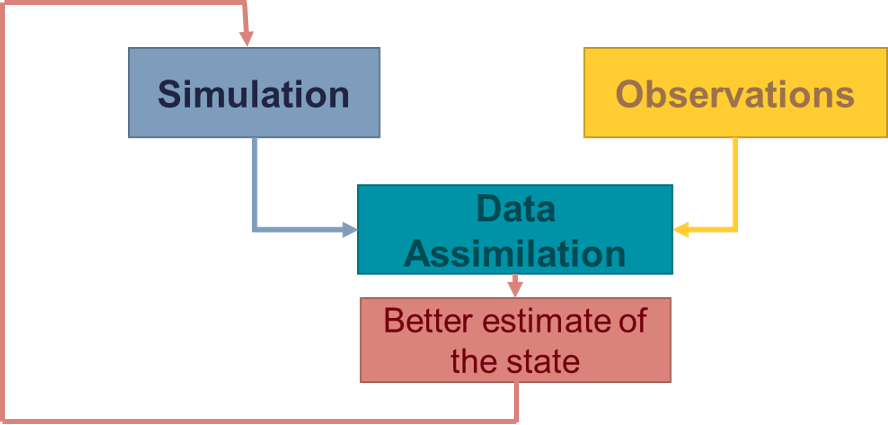
\includegraphics[width=0.5\textwidth]{images/data_assimilation_scheme.png}
    \end{figure}
\end{frame}

\subsubsection{Sequential Filtering - Ensemble Kalman Filter}

\begin{frame}{Sequential Filtering - Ensemble Kalman Filter}
    \small
    We note $u(x, t)$ a field (state) and $y(t)$ the observation with $x$ a spatial variable and $t$ the time.
    \begin{block}{Sequential Filtering}
        Update the field $u$ each time an observation $y$ is made, given a prediction $\hat u$.
    \end{block}
    \vfill
    \begin{block}<2->{Ensemble Kalman Filter}
        \begin{itemize}
            \item Generalization of the \textbf{Kalman Filter} where the state distribution is represented by an \textbf{ensemble} of state in order to estimate statistics and propagate uncertainty~\cite{evensen_sequential_1994}.
            \item Adapted to \textbf{non-linear} and \textbf{high-dimansional} state space.
        \end{itemize}
    \end{block}
\end{frame}

\begin{frame}{Ensemble Kalman Filter}
    \begin{columns}
        \begin{column}{0.6\textwidth}
            \small
            we note $u(\cdot, t_{k}) = u_k(\cdot)$,
            \begin{itemize}
                \item<1-> \textbf{Initialization} \\
                    Sample $N$ fields $\left\{u^i_0\right\}_{i=1}^N \stackrel{iid}{\sim} U_0$
                    \vfill
                \item<2-> \textbf{Forecast} from $t$ to $t_{k+1}$ (e.g. with numerical simulation code) \\
                    $\hat u^i_{k+1} = \mathcal M(u_k^i), \quad i = 1, \dots, N$
                    \vfill
                \item<3-> \textbf{Measurement and prediction} at $t_{k+1}$\\
                    measure $y_{k+1}$, \\
                    prediction $h^i_{k+1} = \mathcal H (\hat u^i_{k+1}) \quad i = 1, \dots, N$
                    \vfill
                \item<4-> \textbf{Analysis} A weighted linear combination of $\hat u_{k+1}^i$ \\
                    $u^i_{k+1} = \hat u^i_{k+1} + \sum_{j=1}^N \bm F_{ij} \hat u^i_{k+1}$, \\ where $\bm F$ depends on $\left(y_{k+1}, \left\{h^i_{k+1}\right\}_{i=1}^N\right)$\footnotemark[1]
            \end{itemize}
        \end{column}
        \begin{column}{0.4\textwidth}
            \begin{figure}
                \centering
                \only<1>{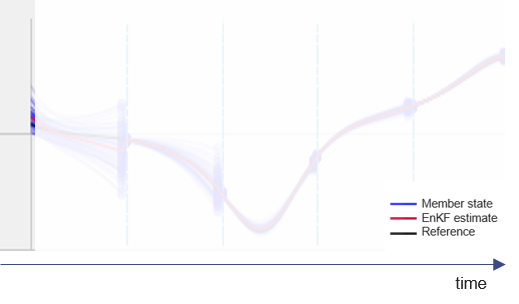
\includegraphics[width=\textwidth]{images/initialization.png}}
                \only<2>{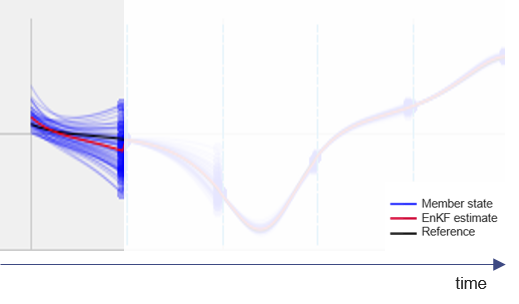
\includegraphics[width=\textwidth]{images/propagation.png}}
                \only<3>{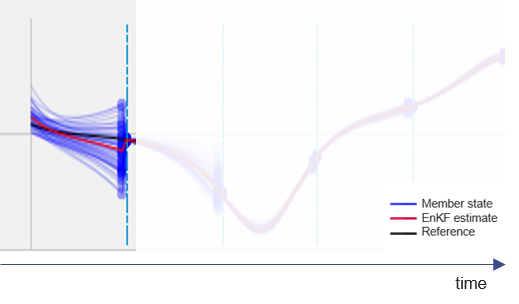
\includegraphics[width=\textwidth]{images/obs_analasis.png}}
                \only<4>{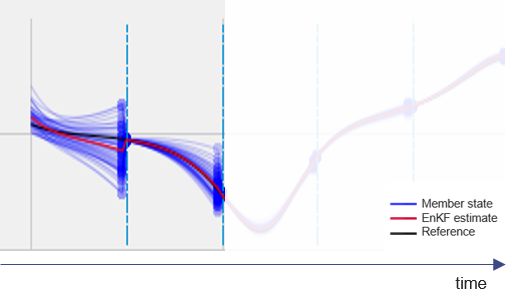
\includegraphics[width=\textwidth]{images/obs_analasis2.png}}
                \only<5>{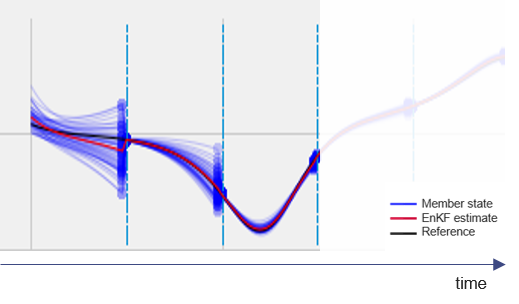
\includegraphics[width=\textwidth]{images/obs_analasis3.png}}
                \only<6>{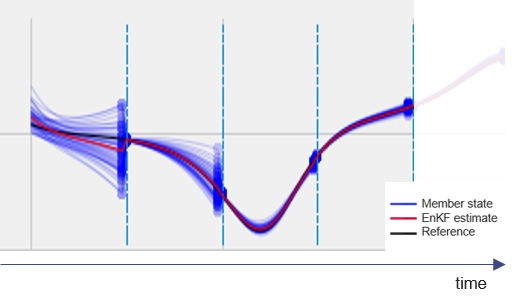
\includegraphics[width=\textwidth]{images/obs_analasis4.png}}
                \only<7>{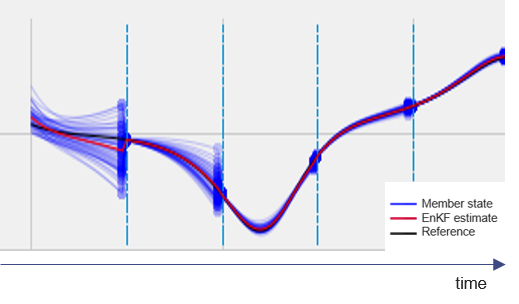
\includegraphics[width=\textwidth]{images/obs_analasis5.png}}
            \end{figure}
        \end{column}
    \end{columns}
    \footnotetext[1]{\tiny equivalent formulation of the original formulation, see~\cite{siripatana_combining_2019}}
\end{frame}

\subsection{Meshless simulation}
\begin{frame}{Meshless simulation}
    \small
    \begin{columns}[t]
        \begin{column}{0.7\textwidth}
            \begin{Definition}
                Meshfree methods - Discretization of $u(x,t)$ thanks to a particle representation \\
                = \textbf{Lagrangian method}
            \end{Definition}
            \begin{itemize}

                \item Particles $p$ : a position $\bm x_p$, an intensity $\Gamma_p$ and a kernel $\phi_h$

                \item The field $u(x, t)$ is discretize with $N_p$ particles such as
                      \begin{equation*}
                          u(x, t) \approx \sum_{p \in \mathcal P} \Gamma_p(t)~\phi_h(x - x_p(t)), \quad \mathcal P = \left\{x_p, \Gamma_p\right\}_{p=1}^{N_p}
                      \end{equation*}
                \item The model evolution
                      \begin{eqnarray*}
                          \frac{d\Gamma_p}{dt} = 0, \quad \frac{d x_p}{d t} = v(x_p; \mathcal P)
                      \end{eqnarray*}
                      $\Rightarrow u_{k+1} = \mathcal M(u_{k})$
            \end{itemize}
        \end{column}
        \begin{column}{0.3\textwidth}
            \begin{figure}
                \begin{subfigure}[t]{\textwidth}
                    \centering
                    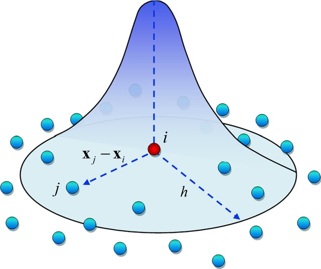
\includegraphics[width=0.5\textwidth]{images/kernel.png}
                    \caption{\tiny kernel function}
                \end{subfigure}
                \centering
                \begin{subfigure}[b]{\textwidth}
                    \centering
                    \animategraphics[loop, autoplay, width=0.8\textwidth]{10}{images/lag_representation/b1da922d43984958b92c8b71e90b82a600e60cucwjbaqV5A-}{0}{35}
                    \caption{\tiny Dipole simulation with Vortex Method.}
                \end{subfigure}
            \end{figure}
        \end{column}
    \end{columns}
\end{frame}

\begin{frame}{EnKF Update with meshless simulation}
    \begin{block}{EnKF Update at $t=t_a$:}
        \begin{itemize}
            \item $u_i(x, t_a) = \hat u_i(x, t_a) + \sum_{l=1}^{N} F_{ij}~\hat u_j(x, t_a), \quad i = 1, \dots, N$ \\
            \item<2-> Find : $u_i(x, t_a) \approx \sum_p \textcolor{ceared}{\Gamma_{p, j}(t_a)}~\phi_h (x - \textcolor{ceared}{x_{p, j}(t_a)}), \quad i = 1, \dots, N$\\
                $\Leftrightarrow$ update the particule discretization: $\mathcal P_i = \left\{x_p, \Gamma_p\right\}_{p=1}^{N_p} \mapsto \mathcal P_i^a = \left\{x_p^a, \Gamma^a_p\right\}_{p=1}^{N^a_p}, \quad i = 1, \dots, N$
        \end{itemize}
    \end{block}
    \vfill

    \only<3->{\textbf{Update}}:
    \begin{itemize}
        \item<3->  \only<1>{Intensities} \only<4->{\textcolor{ceared}{Intensities}}
        \item<3-> Particle Positions
        \item<3-> both
    \end{itemize}
\end{frame}

\section{Intensity correction}
\begin{frame}{Intensity correction}
    $\mathcal{P}_i = \left\{x_p, \textcolor{ceared}{\hat \Gamma_{p, i}}\right\}_{p=1}^{N_p} \mapsto \left\{x_p, \textcolor{ceared}{?} \right\}_{p=1}^{\textcolor{?}}$

    \begin{block}<2->{First case: same particles positions}
        Linear combinaison of intensity $\Gamma_{p,i}$ with the same positions $x_p$\\
        $\left\{x_{p,i}, \hat \Gamma_{p,i}\right\}_{p=1}^{N_p} \mapsto \left\{x_p, \hat \Gamma_{p, i} + \sum_{j=1}^{N_p^j} F_{ij} \hat \Gamma_{p,j} \right\}_{p=1}^{N_p}$
    \end{block}
    \begin{block}<3->{General case: Different particles configurations}
        Combinaison of \textbf{all particles}! \\
        $ \left\{x_{p,i}, \hat \Gamma_{p,i}\right\}_{p=1}^{N^i_p} \mapsto \left\{x_{p,i}, \hat \Gamma_{p,i} + F_{ii}\Gamma_{p,i} \right\}_{p=1}^{N_p^i} + \left[\left\{x_{p,i}, F_{ij} \hat \Gamma_{p,j}\right\}_{p=1}^{N_p^j}\right]_{j\neq i}$ \\
    \end{block}
\end{frame}

\begin{frame}{Remesh EnKF}
    \subtitle{Regrid on a common particle configuration}
    \begin{itemize}
        \item Generate a new regular particle set based on particle-grid operator$\footnotemark[1]$.
              \begin{figure}
                  \centering
                  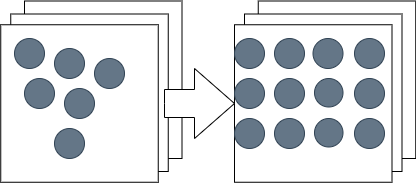
\includegraphics[width=0.5\textwidth]{images/remesh_enkf.png}
                  \caption{remeshing operation. Generate a new regular particle set.}
              \end{figure}
        \item Apply the intensity update on the commun configuration
    \end{itemize}

    \footnotetext[1]{\tiny used by particles-in-cell methods (MPM, VIC,...).}
\end{frame}

\begin{frame}{Part EnKF}
    \subtitle{Project solution on each forecast configuration}
    \begin{itemize}
        \item Keep the previous particles positions $x_{p, i}$
        \item Project the analysed solution on those particles: \\
              \begin{equation*}
                  \Gamma_{p, i} = \langle u, \phi_h(\cdot,x_{p,i})\rangle_{L_2}, \quad p = 1, \dots, N_p^i.
              \end{equation*}
    \end{itemize}
    \vfill
    \centering
    $\left\{x_{p,i}, \hat \Gamma_{p,i}\right\}_{p=1}^{N_p} \mapsto \left\{x_{p,i}, \langle u, \phi_h(\cdot,x_{p,i})\rangle_{L_2} \right\}_{p=1}^{N_p}$
\end{frame}

\section{Position update}
\begin{frame}{Intensity correction - limitation}
    \begin{itemize}
        \item Previous filter only update intensities
        \item Confined to the particle support $\rightarrow$ might be inadequate to the analysis solution

    \end{itemize}

    \begin{figure}
        \centering
        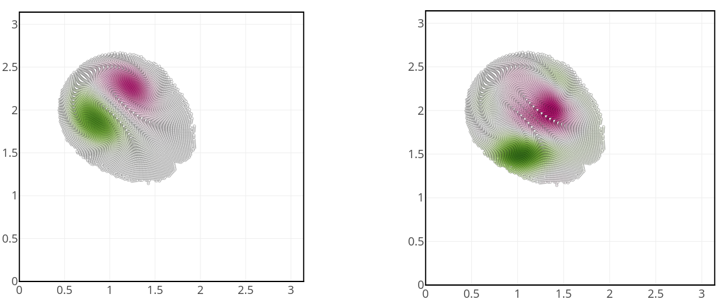
\includegraphics[width=0.5\textwidth]{images/unalign_discretization.png}
        \caption{Left: forecasted particle set, Right: updated particle set.}
    \end{figure}

    \only<2->{\textbf{Update}:}
    \begin{itemize}
        \item<2->Intensities
        \item<2-> \textcolor{ceared}{Particle Positions}
        \item<2-> both
    \end{itemize}
\end{frame}

\begin{frame}{Position update}
    Fitting $u_a$ by changing $x_p$ not an easy task:
    \begin{itemize}
        \item fit an intensity correction with position correction
        \item should be in the Span($\hat u^i$)
        \item non-linear problem of dimension $N_p^i$
    \end{itemize}

    \begin{block}<2->{Our hypothesis}
        Error in the velocity field $v$ lead to error in the integration of the particles position: $\frac{d x_p}{d t} = v(x_p; \mathcal P)$
    \end{block}

    \begin{block}<3->{Goal}
        Correct the particles position $x_p$ of the forecast field $\hat u$ by integrating a velocity field to reduce directly the discrepency between \textbf{prediction} and the \textbf{observations}
    \end{block}
\end{frame}

\begin{frame}{Position correction}
    \begin{block}{Goal}
        Correct the particles position $x_p$ of the forecast field $\hat u$ by integrating a velocity field to reduce directly the discrepency between \textbf{prediction} and the \textbf{observations}:
        \begin{equation*}
            \min_{v_c \in \mathcal V} \left\|d - h_{v_c}(\hat u(\cdot); v_c) \right\|^2 \only<2->{\textcolor{ceared}{+ R(v_c)}}, \quad i = 1, \dots, N
        \end{equation*}
    \end{block}
    \only<2->{$\textcolor{ceared}{R(v_c)}$ is a regularisation term. (avoid non-unicity and ill-conditioning)}

    \begin{block}<3->{Position transformation $\Phi$: integration of the correction field $v_c$}
        \begin{equation*}
            \Phi(x_p; v_c) = x_p + \int_{0}^{1} v_c(x_p(t))~\mathrm{d}t \Rightarrow \left\{\textcolor{ceared}{x_{p,i}}, \hat \Gamma_{p,i}\right\}_{p=1}^{N^i_p} \mapsto \mathcal{P}_{i, \Phi} = \left\{\textcolor{ceared}{\Phi(x_{p,i}; v_c)}, \hat \Gamma_{p,i}\right\}_{p=1}^{N^i_p}
        \end{equation*}
    \end{block}
\end{frame}

\begin{frame}{Formulation}

    \begin{block}{Searching space}
        Need to be an incompressible field to be physically consistent $\Rightarrow \nabla $ \\
        We search the velocity as a linear combination of member velocity field  \\
        $\Rightarrow v_c \in \mathrm{Span}\left(\{v_i\}_{i=1}^{N}\right) \Rightarrow$ $v_c = \sum_{i=1}^N a_i v_i, \quad a_i \in \mathbb{R}$.
    \end{block}

    \vfill
    \only<2->{Finally $N$ independant problems of dimension $N$ to solve:  \\

        \begin{equation*}
            \mathcal L_i (a) = \min{a \in \mathbb{R}^N} \left\|d - h_a(\hat u_i(\cdot); a) \right\|^2 + \lambda \|a\|^2, \quad i = 1, \dots, N
        \end{equation*}
        \vfill
        By estimating $\nabla_a h_a$ we deduce $\nabla_a \mathcal L_i \rightarrow$ local gradient optimizer (BFGS).}
\end{frame}

\begin{frame}{Problem}
    \begin{itemize}
        \item We solve the Euler equation for incompressible fluid flow with the \textbf{Vortex Method}~\footnotemark[1]
        \item The particle set discretizes the vorticity field $\omega = \nabla \cdot v$
        \item Three vortex(body) problem: chaotic trajectory~\footnotemark[2]
        \item Ensemble: perturbed position, amplitude, core-size of vortex
    \end{itemize}

    \begin{figure}
        \begin{subfigure}[t]{0.32\textwidth}
            \centering
            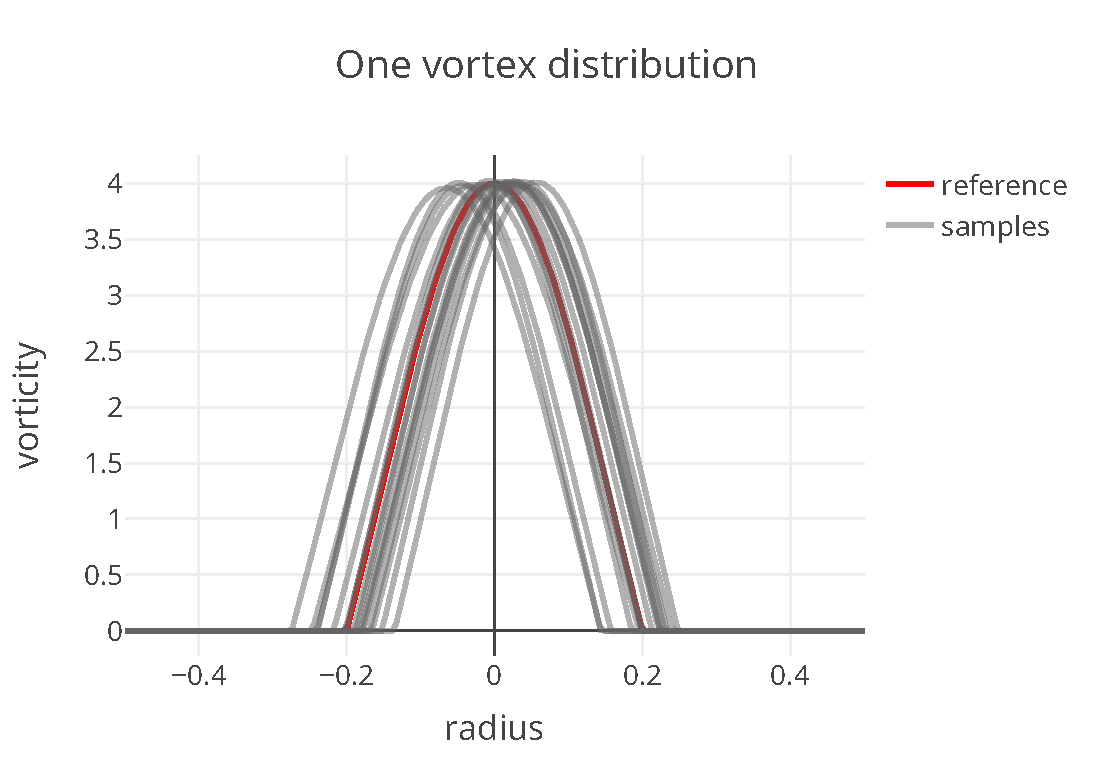
\includegraphics[width=\textwidth]{images/vortex_distribution.pdf}
            \caption*{\tiny Reference and samples set of one vortex}
        \end{subfigure}
        \begin{subfigure}[t]{0.32\textwidth}
            \centering
            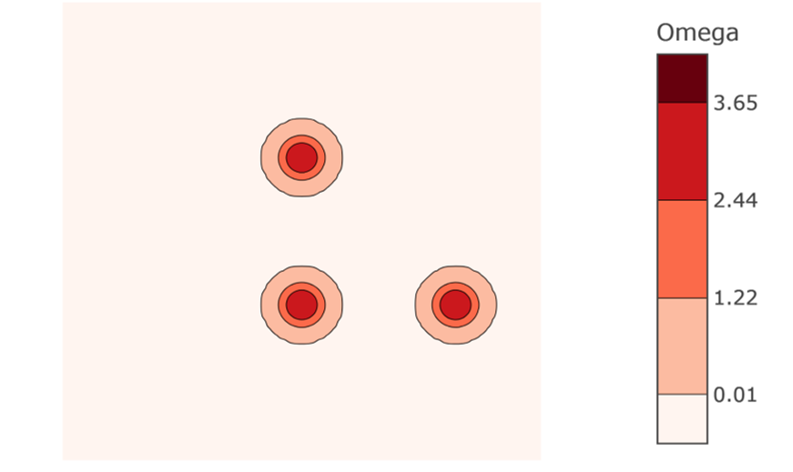
\includegraphics[width=\textwidth]{images/vorticity_field.png}
            \caption*{\tiny Vorticity field of the three vortex at $t=0$}
        \end{subfigure}
        \begin{subfigure}[t]{0.32\textwidth}
            \centering
            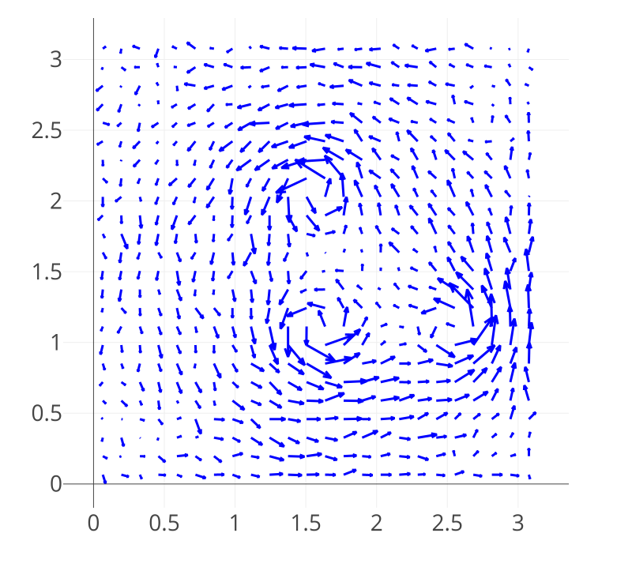
\includegraphics[width=0.8\textwidth]{images/obs_velocity.png}
            \caption*{\tiny Observed induced velocity field at $t=0$}
        \end{subfigure}
    \end{figure}

    \footnotetext[1]{\tiny \cite{cottet_vortex_2000}}
    \footnotetext[2]{\tiny \cite{aref_motion_1979}}
\end{frame}

\begin{frame}{Without assimilation}
    \begin{columns}
        \begin{column}{0.5\textwidth}
            \begin{figure}[t]
                \centering
                \animategraphics[loop, autoplay, width=0.8\textwidth]{10}{images/non_assim_traj/f534a289c8aa420ab3f6d5c7d5f2214583FIwJoqDx6i0hPj-}{0}{73}
                % \caption*{Vortex center trajectories}
            \end{figure}
        \end{column}
        \begin{column}{0.5\textwidth}
            \begin{figure}
                \centering
                \begin{subfigure}{\textwidth}
                    \centering
                    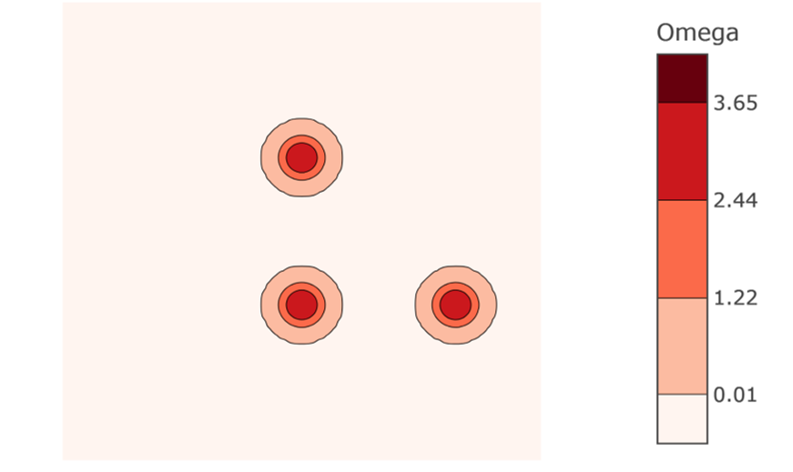
\includegraphics[width=0.8\textwidth]{images/vorticity_field.png}
                    % \caption*{Vortex position error}
                \end{subfigure}
                \begin{subfigure}{\textwidth}
                    \centering
                    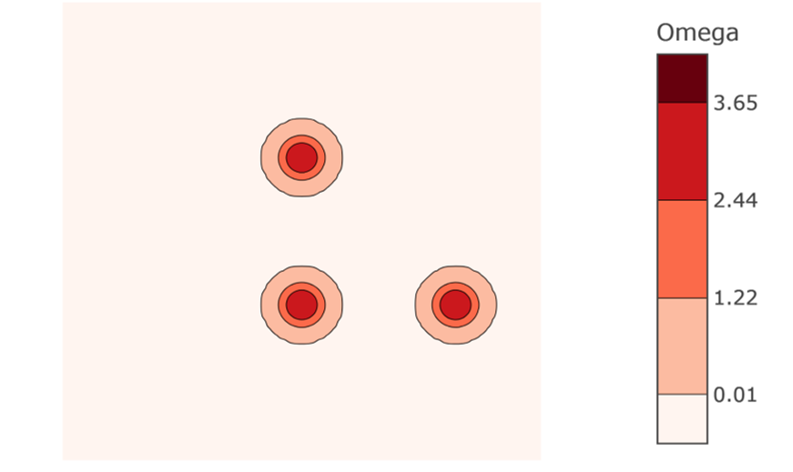
\includegraphics[width=0.8\textwidth]{images/vorticity_field.png}
                    % \caption*{Vorticity error}
                \end{subfigure}
            \end{figure}
        \end{column}
    \end{columns}
\end{frame}

\begin{frame}{With assimilation}
    \begin{columns}
        \begin{column}{0.5\textwidth}
            \begin{figure}
                \centering
                \begin{subfigure}{\textwidth}
                    \centering
                    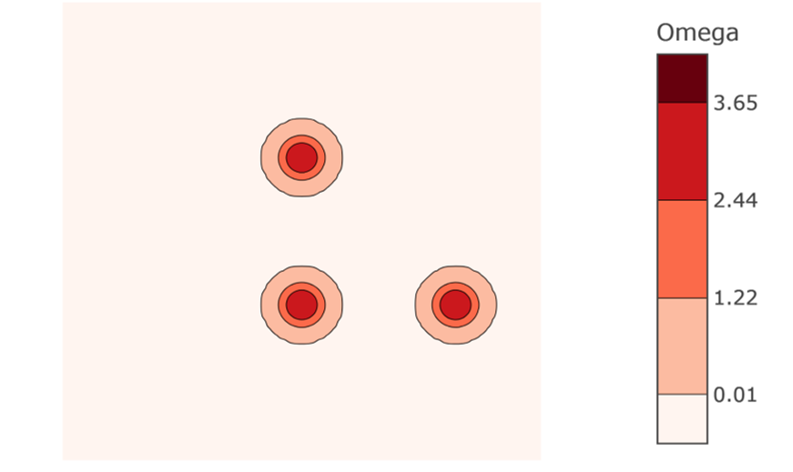
\includegraphics[width=\textwidth]{images/vorticity_field.png}
                \end{subfigure}
                \begin{subfigure}{\textwidth}
                    \centering
                    \animategraphics[loop, autoplay, width=0.8\textwidth]{10}{images/assim_trajectories/3651ba82007d4ae5e7ae2e592eed1014BZkA9i3epEQadmQl-}{0}{73}
                \end{subfigure}
            \end{figure}
            % \caption*{Vortex center trajectories}
        \end{column}
        \begin{column}{0.5\textwidth}
            \begin{figure}
                \centering
                \begin{subfigure}{\textwidth}
                    \centering
                    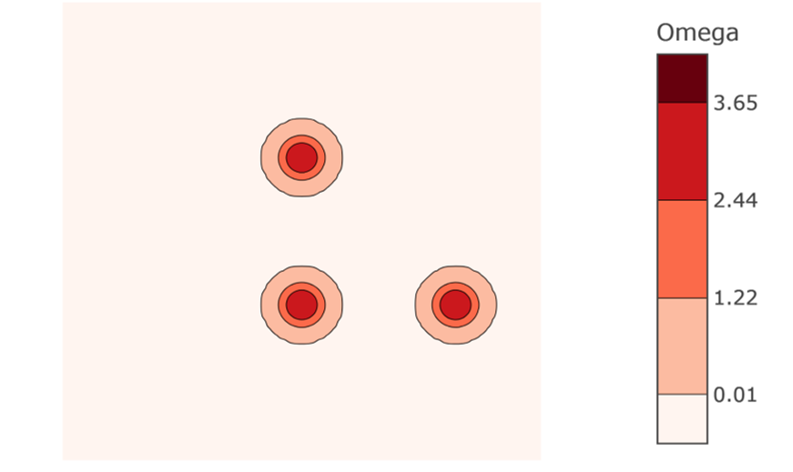
\includegraphics[width=\textwidth]{images/vorticity_field.png}
                    % \caption*{Vortex position error}
                \end{subfigure}
                \begin{subfigure}{\textwidth}
                    \centering
                    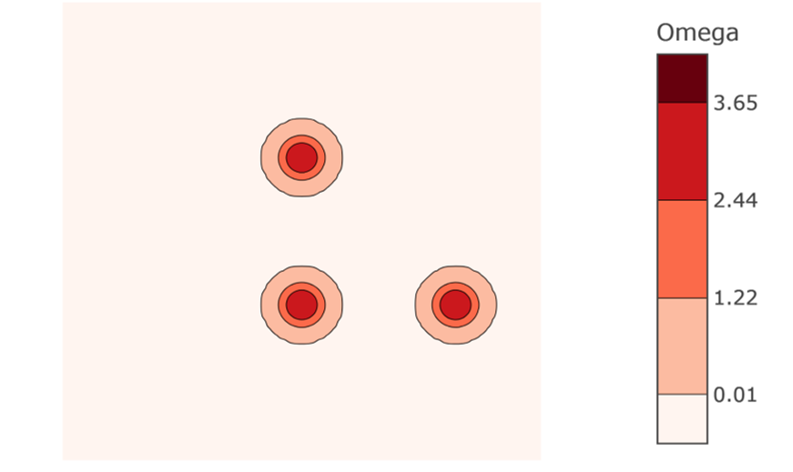
\includegraphics[width=\textwidth]{images/vorticity_field.png}
                    % \caption*{Vorticity error}
                \end{subfigure}
            \end{figure}
        \end{column}
    \end{columns}
\end{frame}

\begin{frame}{Discussions and Perspectives}

    \begin{block}{Discussions}
        \begin{itemize}
            \item Adapted the EnKF update for meshless simulations based on intensity update
            \item Introduce a formulation to correct particle position
        \end{itemize}
    \end{block}

    \begin{block}{Perspectives}
        \begin{itemize}
            \item Proposed a combined formulation
        \end{itemize}
    \end{block}
\end{frame}

\closingframe

\begin{frame}[allowframebreaks, noframenumbering]
    \frametitle{References}
    \printbibliography % Print the bibliography
\end{frame}

% \section*{Addendum}
% \begin{frame}{EnKF update}
%     \emph{Be successful with your presentation!}
% \end{frame}

\end{document}
